% !TEX program = xelatex
\documentclass[14pt]{beamer}

\usepackage{amsmath}
\usepackage{fouriernc}
\usefonttheme{professionalfonts}

\usepackage{bxdpx-beamer}
\usetheme[progressbar=frametitle,numbering=fraction]{metropolis}

\usepackage{zxjatype}
\setsansfont[Scale=0.85]{Roboto Medium}
\setjasansfont[Scale=0.81]{Noto Sans CJK JP Medium}

\usepackage{bm}
\usepackage{color}
% \usepackage{listings,jlisting}
\usepackage{listings}
\lstset{language={C}, basicstyle=\ttfamily\footnotesize,
  commentstyle=\textit, classoffset=1, frame=tRBl, framesep=5pt,
  numbers=left, stepnumber=1, numberstyle=\footnotesize, tabsize=2 }
% \usepackage{slashbox}
\usepackage{hyperref}

\usepackage{graphicx}
\graphicspath{ {./images/} }
\usepackage{subcaption}

\usepackage{makecell}

\usepackage{ruby} %日本語ルビ。xelatex も OK!

\title{オンライン沖縄語辞典}
\author{中村 仁宣 (Hisanobu Nakamura)}
\begin{document}
\begin{frame}
  \maketitle  
\end{frame}

\section{自己紹介}

\begin{frame}{初めてぃうがなびら!}
  はいさい、\ruby{初}{はじ}めてぃうがなびら!わんねー...
    \begin{itemize}
    \item \ruby{名前}{のーじ}や\textbf{\ruby{中村仁宣}{なかむら ひさのぶ}}んでぃ\ruby{言}{い}ちょーいびーん。
    \item \ruby{出身}{すだち}や\textbf{愛知県名古屋市}やいびーん。イギリスんかいん\ruby{暮}{く}らちょーたる\ruby{事}{くとぅ}んあいびーん。
    \item 2021年に\ruby{那覇}{なーふぁ}うてぃ\ruby{暮}{く}らし\ruby{始}{はじ}みびたん。
    \item 大学・大学院うとーてぃ専攻さる分野や\textbf{数学・物理}やいびーたん。
    \item 前職や\textbf{機械学習エンジニア}やいびーたん。
    \item \ruby{言語}{くとぅば}\ruby{習}{なら}いしぇー\ruby{好}{し}ちやいびーん。
    \end{itemize}
\end{frame}

\begin{frame}{はじめに}
  今日、話す内容は、元々沖縄に縁がなかった登壇者が、沖縄語を学習するにあたり体験した困難と、持ち合わせていたプログラミングの知識を使ってそのほんの一部を自分なりに解決したストーリーについてです。
  よって、この話は
  \begin{enumerate}
  \item \ruby{一}{いち}沖縄語学習者としての視点
  \item ツールの作成者としての視点
  \end{enumerate}
  の2つの視点から書かれています。このお話が、マイノリティ言語の新規学習者に対してどのように情報発信、または学習環境の整備等をすれば良いかのヒントになれば、と思っております。
\end{frame}

\begin{frame}{今日話す内容}
  \begin{enumerate}
  \item オンライン沖縄語辞典開発の経緯
  \item オンライン沖縄語辞典の紹介
  \item 得られた知見
  \item 今後の展望
  \end{enumerate}
\end{frame}

\section{オンライン沖縄語辞典開発の経緯}

\begin{frame}{オンライン沖縄語辞典開発の経緯}
  \begin{block}{開発者が沖縄語学習を開始}
    \begin{itemize}
    \item  2021年6月に那覇に移住。
    \item  2022年6月に沖縄語学習を始める。
    \item  教材・辞書を探し始めるが、選択肢は少ない。
    \item  Web上で使える辞典は、カジュアル・断片的なものが多い。
    \end{itemize}
  \end{block}
\end{frame}

% \begin{frame}{オンライン沖縄語辞典開発の経緯}
%   \begin{block}{現在、入手しやすい(?)辞書}
%     \begin{table}[ht]
%       \begin{tabular}{|c|c|c|} 
%         \hline
%         題名/出版元(発刊年) & 語彙数 & 値段  \\ [0.5ex] 
%         \hline\hline
%         沖縄語辞典/研究社(2006) & 8,000 & ¥3,200  \\
%         \hline
%         沖縄語辞典/NINJAL$^*$(1963) & 約12,000 & ¥15,000〜  \\
%         \hline
%         琉球語辞典/大学書林(1999) & 約12,000 & ¥26,000〜 \\
%         \hline
%         \hline
%       \end{tabular}
%     \end{table}
%     *NINJAL=国立国語研究所
%   \end{block}
% \end{frame}

% \begin{frame}{オンライン沖縄語辞典開発の経緯}
%   \begin{block}{}
%     \begin{itemize}
%     \item 沖縄語辞典/国立国語研究所(NINJAL)(1963), 約12,000, ¥15,000〜 
%     \end{itemize}
%     \end{table}
    
%   \end{block}
% \end{frame}


\begin{frame}{オンライン沖縄語辞典開発の経緯}
  \begin{block}{『沖縄語辞典』と『うちなーぐち活用辞典』}
    \begin{itemize}
    \item 沖縄語辞典、国立国語研究 出版、1963年発行、約12000語、¥15,000〜
    \item うちなーぐち活用辞典、編・著者 宮良信詳、国立国語研究所 言語変異研究領域、2021年発行
    \end{itemize}
  \end{block}
\end{frame}

\begin{frame}{オンライン沖縄語辞典開発の経緯}
  \begin{block}{価値}
    \begin{itemize}
    \item 『沖縄語辞典』
      \begin{itemize}
      \item 豊富な語彙数、例文、用言活用の解説等を含む。
      \item 士族・平民発音の区別。古い言葉・意味の記載。
      \end{itemize}
    \item 『うちなーぐち活用辞典』
      \begin{itemize}
      \item 現代の沖縄語の豊富な例文を含む。
      \end{itemize}
    \end{itemize}
  \end{block}  
\end{frame}


\begin{frame}{オンライン沖縄語辞典開発の経緯}
  \begin{block}{NINJAL データにたどり着く}
    \begin{itemize}
    \item 紙の『沖縄語辞典』『うちなーぐち活用辞典』を入手するが、重さのため持ち運べず。
    \item このような語彙数・例文などが豊富なオンライン辞典があればいいのになと思う。
    \item NINJAL で『沖縄語辞典』の \textbf{Excel データがダウンロード可能}だと知る。
    \item ないのなら、『沖縄語辞典』のデータを\textbf{オンライン上で簡単に検索できるようにすれば良い!}
    \item どうせ作るのなら、\textbf{他の人にも使って貰いたい}。      
    \end{itemize}
  \end{block}
\end{frame}

\begin{frame}{オンライン沖縄語辞典開発の経緯}
  \begin{block}{開発の開始}
    \begin{itemize}
    \item しかし、Excel のデータをそのまま使ったのでは、一般ユーザーにとっては使いにくい所もある...
    \end{itemize}
  \end{block}
  \begin{figure}[ht]
    \centering
    \includegraphics[height=0.36\paperheight]{okinawago-app-early-page.jpeg}
    % \begin{minipage}{0.3\paperwidth}
    %   % \caption{PDF}
    % \end{minipage}
  \end{figure}
\end{frame}

\begin{frame}{オンライン沖縄語辞典開発の経緯}
  \begin{block}{『沖縄語辞典』を使う上でのハードル}
    \vspace{0pt}
    音素記号を知らない利用者、初級学習者、などの一般ユーザーにとって、、、
    \begin{enumerate}
    \item 音素記号を知らないと\textbf{使う事ができない}(検索も例文を読むこともできない)
      \begin{itemize}
      \item 沖縄語は音素記号のみの表記。
      \end{itemize}
    \item 「解説篇」を読まないと\textbf{動詞活用がわからない}
      \begin{itemize}
      \item 動詞の活用は自分で考える必要がある。
      \end{itemize}
    \item \textbf{初見では解読困難な知識が必要}。
    \item 語彙の説明文の空白が圧縮されていて\textbf{読みづらい}
    \end{enumerate}
  \end{block}
\end{frame}

\begin{frame}{オンライン沖縄語辞典開発の経緯}
  \begin{block}{電子情報の利点を活かす}
    \vspace{0pt}
    『沖縄語辞典』は、元々紙の辞書として作成され、紙面の節約の必要性があるため、重複を省き、変化部分のみを記す経済的な表記法にならざるをえないが、電子空間上ではその制限は緩くなり、わかり易さのための冗長性を(許容範囲内で)持たせられる。テキスト処理とWeb技術でそれが可能。
  \end{block}
\end{frame}

\begin{frame}{オンライン沖縄語辞典開発の経緯}
  \begin{block}{『沖縄語辞典』をより多くの人へ}
    \vspace{0pt}
    そこで、以下の点を情報技術により克服することで、より多くの人にとって使いやすいオンライン沖縄語辞典を作る事を目標とした。
    \begin{enumerate}
    \item 音素記号をカナとIPAで表示する。
    \item 語彙説明の中の沖縄語もカナ表示する。
    \item 動詞の活用表を自動で生成する
    \end{enumerate}
  \end{block}
\end{frame}

\section{オンライン沖縄語辞典}

% \begin{frame}{オンライン沖縄語辞典}
%   \begin{block}{オンライン沖縄語辞典}
%     \begin{figure}[ht]
%       \centering
%       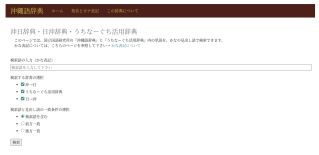
\includegraphics[height=0.5\paperheight,width=0.7\paperwidth]{okinawago-app-top-page.png}
%     \end{figure}
%   \end{block}
% \end{frame}

\begin{frame}{オンライン沖縄語辞典}
  \begin{block}{概要}
    \begin{itemize}
    \item  収録辞書:『沖縄語辞典』(沖日、日沖)、『うちなーぐち活用辞典』
    \item  URL:https://okinawago.app/
    \item 使用料:なし
    \end{itemize}
    \begin{figure}[ht]
      \centering
      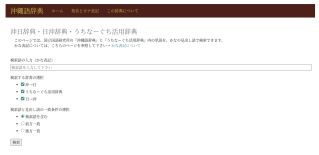
\includegraphics[height=0.35\paperheight,width=0.5\paperwidth]{okinawago-app-top-page.png}
    \end{figure}
  \end{block}
\end{frame}

\begin{frame}{オンライン沖縄語辞典}
  % 検索の画像
  \begin{block}{検索の仕方と結果}
  \end{block}
\end{frame}

\begin{frame}{オンライン沖縄語辞典}
  % 比較の画像
  \begin{block}{動詞「アーキユン」での文章表示比較}
    \begin{figure}[ht]
      \centering
      \begin{minipage}{0.5\textwidth}
        \includegraphics[height=0.5\paperheight,width=0.4\paperwidth]{oki-dict-example-aakiyun-original.png}
        %\caption{PDF}
      \end{minipage}%
      \begin{minipage}{0.5\textwidth}
        \includegraphics[height=0.65\paperheight]{oki-dict-example-aakiyun-online.png}
        %\caption{オンライン沖縄語辞典}
      \end{minipage}
    \end{figure}
  \end{block}
\end{frame}

% \begin{frame}{オンライン沖縄語辞典}
%   \begin{block}{音素記号$\rightarrow$カナ・IPA変換}
%     \begin{itemize}
%     \item 沖縄語音素表記を音節に分解し、カナとIPAに変換する処理を実装。
%     \item カナ検索では可能な限り多様な表記法に対応
%     \item 士族発音がある場合は併記。(「解説篇」を参照した)
%     \item 副産物として、沖縄語音素表記の誤表記を検出できるようになった。
%     \end{itemize}
%   \end{block}
% \end{frame}

\begin{frame}{オンライン沖縄語辞典}
  % カナ表示について
  \begin{block}{カナ表記について}
    \vspace{0pt}
    開発者が今まで見かけた中で、取り入れやすい表記法をできるだけ多くのバリエーションで検索できるように努力した。
    「どれか一つでしか検索できない」ではなく、「どの表記法でも検索できる」を目指したかった。
  \end{block}
\end{frame}

\begin{frame}{オンライン沖縄語辞典}
  % カナ表示について
  \begin{block}{カナ表示の例}
    \begin{figure}[ht]
      \centering
        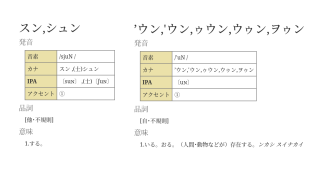
\includegraphics[height=0.6\paperheight,width=0.9\paperwidth]{okinawago-app-pronunciation-example2.png}
    \end{figure}
  \end{block}
\end{frame}

\begin{frame}{オンライン沖縄語辞典}
  % カナ表示について
  \begin{block}{カナ表記について}
    \vspace{0pt}
    参考にした書籍、文献
    \begin{itemize}
    \item 『沖縄語入門』
    \item 『初級 沖縄語』
    \item 研究社『沖縄語辞典』
    \item 沖縄県の『沖縄県における「しまくとぅば」の表記について』
    \item しまくとぅば普及協議会の教材
    \end{itemize}
  \end{block}
\end{frame}

% \begin{frame}{オンライン沖縄語辞典}
%   \begin{block}{語彙説明文と沖縄語例文の分離}
%     \begin{itemize}
%     \item 解説文の日本語パラグラフと沖縄語例文(音素表記)とを分解する処理を実装。
%     \item ユニットテストと音素カナ変換のエラー検知機能を使いトライ&エラーで適切な正規表現を作成。
%     \item 「ほとんど」の例文を分離できているが、一部できていない箇所もあるかもしれない。正規表現による正確な処理は対象データに対する網羅的な知識が必要。
%     \end{itemize}
%   \end{block}
% \end{frame}

\begin{frame}{オンライン沖縄語辞典}
  \begin{block}{語彙説明文と沖縄語例文の分離}
    \begin{figure}[ht]
      \centering
      \begin{minipage}{\paperwidth}
        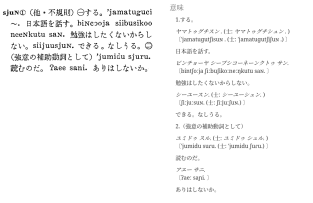
\includegraphics[height=0.6\paperheight,width=0.7\paperwidth]{okinawago-app-explanation-example.png}
        %\caption{士族発音}
      \end{minipage}
    \end{figure}
  \end{block}
\end{frame}

\begin{frame}{オンライン沖縄語辞典}
  \begin{block}{語彙説明文と沖縄語例文の分離}
    \begin{itemize}
    \item 「ほとんど」の例文を分離できているが、一部できていない箇所もあるかもしれない。
    \item 正規表現による処理を行っているため、正確な処理は対象データに対する網羅的な知識が必要。
    \end{itemize}
  \end{block}
\end{frame}

\begin{frame}{オンライン沖縄語辞典}
  \begin{block}{動詞活用表の例}
    \begin{figure}[ht]
      \centering
      \begin{minipage}{0.4\paperwidth}
        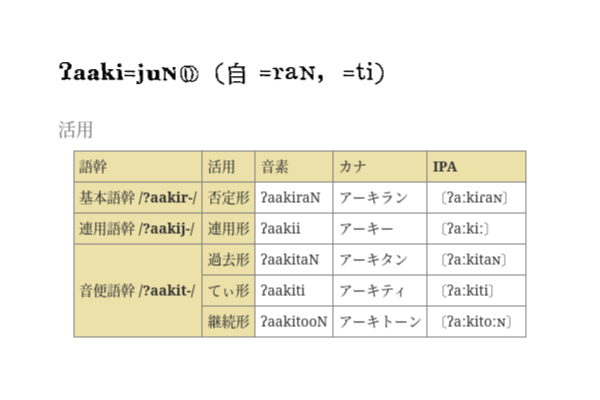
\includegraphics[height=0.36\paperheight]{verb-conugation-comparison.png}
        %\caption{PDF}
      \end{minipage}%
      \begin{minipage}{0.4\textwidth}
        \includegraphics[height=0.34\paperheight]{verb-conjugation-comparison-2.png}
        %\caption{オンライン沖縄語辞典}
      \end{minipage}
    \end{figure}
  \end{block}
\end{frame}

\begin{frame}{オンライン沖縄語辞典}
  \begin{block}{動詞活用表の生成について}
    \begin{itemize}
    \item 元の『沖縄語辞典』では品詞の部分に否定形とティ形語幹末尾のみの記載だった。
    \item 不規則動詞の活用辞書を手で作成。規則動詞は自動生成。
    \end{itemize}
  \end{block}
\end{frame}

%---------  うちなーぐち活用辞典 ----------% 
% \begin{frame}{オンライン沖縄語辞典}
%   \begin{block}{うちなーぐち活用辞典の取り込み}
%     \begin{itemize}
%     \item 沖縄語(うちなーぐち)の例文を収録。
%     \end{itemize}
%     \begin{figure}[ht]
%       \centering
%       \begin{minipage}{0.4\paperwidth}
%         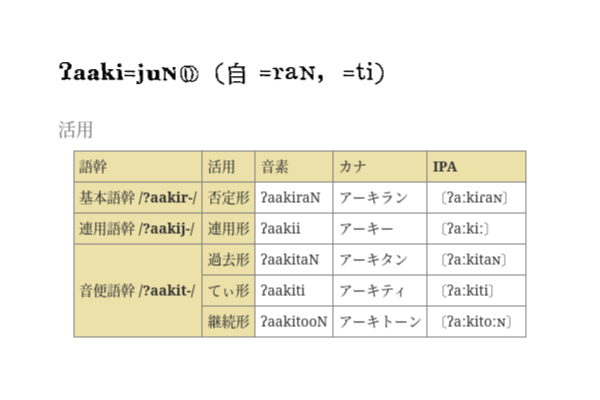
\includegraphics[height=0.36\paperheight]{verb-conugation-comparison.png}
%         %\caption{PDF}
%       \end{minipage}%
%     \end{figure}
%   \end{block}
% \end{frame}

\begin{frame}{オンライン沖縄語辞典}
  \begin{block}{うちなーぐち活用辞典に関する課題}
    \vspace{0pt}    
    PDF の構造化されていないデータを文字のフォント・色・位置・大きさなどの情報から手動で構造化を行った。そのため、まだ正しく構造化できていない箇所がある。
  \end{block}
\end{frame}

\begin{frame}{まとめ1}
  \begin{block}{ユーザビリティ向上のための施策}
    \begin{enumerate}
      \item シンプルで、一貫性のあるページデザイン
      \item カナ表記の解説ページへのリンク
      \item カナで検索可能に。
        \begin{itemize}
        \item 可能な限り多様な表記法に対応
        \end{itemize}
      \item 士族発音も併記
      \item 語彙説明文内の沖縄語の例文の分離。
      \begin{itemize}
      \item 語彙説明文内の沖縄語の例文もカナで表示可能に。
      \item 改行を挿入する事で、視認性も向上。
      \end{itemize}
    \item 動詞活用表の生成。
    \end{enumerate}
  \end{block}
\end{frame}

\begin{frame}{まとめ2}
  \begin{block}{到達しやすさへの施策}
    \begin{enumerate}
    \item シンプルなURL
      \begin{itemize}
      \item URL を覚えてもらえる。チラシに乗せる時にコンパクト。
      \end{itemize}
    \item twitter アカウントとチラシ作り
      \begin{itemize}
      \item SNSでの発信と対面での配布、店舗に配置
      \end{itemize}
    \item QR-code 掲載
      \begin{itemize}
      \item スマートフォンなどで、隣の人にすぐにURLをシェアなどできる
      \end{itemize}
    \end{enumerate}
  \end{block}
\end{frame}

% ---------  知見 ----------%
\section{得られた知見}
\begin{frame}{開発から得た知見}
  \begin{block}{アクセシビリティ(accessibility)の重要性}%
    \vspace{0pt}
    アクセシビリティ := アクセスのしやすさとは...
    \begin{itemize}
    \item 見つけやすさ(searchability)
      \begin{itemize}
      \item 見つけやすい場所にある。
      \end{itemize}
    \item 入手しやすさ(reachability)
      \begin{itemize}
      \item 普通の人が普通の手段・コストで手に入れられる事。
      \end{itemize}
    \item 使いやすさ(usability)
      \begin{itemize}
      \item 使いこなすのに特別な訓練を必要としない事。
      \end{itemize}
    \item \textbf{利用する側からの視点が重要。}
    \end{itemize}
  \end{block}
\end{frame}
\begin{frame}{開発から得た知見}
  \begin{block}{XXにとって利用しやすいデータとは}
    \begin{itemize}
    \item 一般ユーザーにとって
      \begin{itemize}
      \item インターネットなら、検索にヒットしやすい、雑多な劣化した情報に埋もれていない。        
      \item 紙の書籍なら、街の本屋で購入可能である、図書館にある、高くない等
      \item 利用料が相応、または無料。
      \item スマホ・PC上で、カナで検索できる等
      \end{itemize}
    \item 開発者にとって
      \begin{itemize}
      \item データがダウンロード可能で、ある程度構造化(Excel, CSV, JSON, etc)されている。
      \item ソースコードがレポジトリで公開されている。
      \end{itemize}
    \end{itemize}
  \end{block}
\end{frame}
% --------- 展望 ----------%
\section{今後の展望}
\begin{frame}{今後の展望}
  \begin{block}{アプリの改良・充実}
    \begin{itemize}
    \item 辞書機能の充実(活用表の充実、お気に入り語彙、履歴、モバイルアプリ化等)
    \item 学習サポート機能(動詞活用練習、語彙暗記テスト等)
    \item 他辞書の取り込み(さらなる沖縄語、琉球諸語の辞書の追加)
    \item Wiki 作成
    \item 共同開発者・資金調達
    \end{itemize}
  \end{block}
\end{frame}
%--------- 終わり ----------% 
\begin{frame}{終わい}
  \begin{center}
  \LARGE{\ruby{終}{う}わいまでぃ\ruby{聞}{ち}ち\ruby{呉}{くぃ}みそーち\\いっぺー\ruby{御拝}{にふぇー}でーびる。}
  \end{center}
\end{frame}
\end{document}

% \begin{frame}{オンライン沖縄語辞典}
%   \begin{block}{バックエンド}
%     \begin{itemize}
%     \item 『沖縄語辞典』 Excelデータを\textbf{JSON}形式に変換したものを、サーバー上に保持。
%     \item Python の Webアプリケーションフレームワーク Flask 
%     \item GCP(Google Cloud Platform) 上でデプロイ
%     \end{itemize}
%   \end{block}
% \end{frame}

% \begin{frame}{オンライン沖縄語辞典の紹介}
%   \begin{block}{その他のWeb上の教材・辞書}
%     \begin{table}[ht]
%       \resizebox{\textwidth}{!}{% use resizebox with textwidth      
%       \begin{tabular}{|c|c|c|} 
%         \hline
%         サイト & 提供物 & コメント  \\ [0.5ex] 
%         \hline\hline
%         しまくぅば普及協議会& 電子教材・単語帳 & 琉球諸語の挨拶・日常フレーズ集、単語集など。\\
%         \hline
%         琉和辞典 & 沖日・日沖辞典 & \makecell{『沖縄語辞典』の一部の語彙を収録。検索機能なし。\\(http://ryuwajiten.o-ki-na-wa.com/V1.htm)}\\
%         \hline
%         読谷村史資料室 & しまくとぅば単語一覧 & \makecell{読谷地域の語彙集。\\ https://yomitan-sonsi.jp/kana/ta/}\\
%         \hline
%         JLect & 沖日辞典 & \makecell{英語サイト。『沖縄語辞典』、他琉球諸語、\\
%         日本語のその他の方言収録。\\
%         https://www.jlect.com/} \\
%         \hline
%         \hline
%       \end{tabular}
%       }
%     \end{table}
%   \end{block}
% \end{frame}

